\chapter{Experimental Evaluation}
\label{chap:experiment}
We have built our DRS for the QEMU-KVM hypervisor. It uses the \textit{libvirt} APIs for managing the virtual machines and \textit{Openstack} \cite{openstack} mainly for cloud management and software defined networking along with live-migration support. For the distributed key-value store, we use \textit{etcd} \cite{etcd}. We have conducted several experiments to determine the effectiveness of our DRS. The experiments relating to monitoring and auto-ballooning aspect of the DRS have been described below.

\section{Experimental Setup}
Our experimental setup consists of six physical machines. Each physical machine has an 8 core Intel Core i7 3.5GHz CPU, 16 GB memory, 1Gbps NIC and runs the 64 bit Ubuntu 14.04 with Linux kernel version 3.19 . We have installed Openstack on these 6 nodes such that one of the nodes is the controller node(runs the Openstack management services) and the other five are the compute nodes (run the actual VMs). The nodes are connected to a gigabit local network, which they use for transferring data while live migration and for communicating with the outside network. The disks of all the VMs reside on a shared NFS server, and hence, live migration needs to just transfer the memory of the VM between the hosts, and not the disks. Each of the compute nodes also run the DRS software created by us. The controller and two separate nodes (separate from the controller and the compute nodes) run etcd, with a cluster size of three, which provides a fault tolerance of degree one \cite{etcd-ad}. All the VMs that we use run 64 bit Ubuntu 12.04 cloud image. The VMs can be of two sizes - 1 vCPU with 2 GB RAM(small) or 2 vCPU with 4 GB RAM(large).

There are three types of workloads run by these VMs. One workload is memory intensive, one is CPU intensive and one of the workloads is a mix of the two. The memory intensive workload is a program written by us which consumes a total of 1800MB. The program runs in two phases - the allocation phase and the retention phase. The allocation phase starts when the program starts. In the allocation phase, the program tries to allocate 100MB memory using \textit{malloc} and then sleeps for two seconds. This step is performed iteratively till the allocated memory has reached 1800MB. Notably, it may take more than 18 iterations for the allocation to reach 1800MB because malloc will return \textit{null} if it cannot allocate memory due to shortage of memory and the program will sleep for two more seconds. So, the length of the allocation phase depends on the availability of memory. After the allocation phase, retention phase starts, where the program retains the allocated memory for 300 seconds, and does no more allocations. After the retention phase, the program ends. We will refer to this workload as \textit{usemem}.

For the other two types of workloads, we have chosen two SPEC CPU 2006 V1.2 benchmarks \cite{Henning:2006:SCB:1186736.1186737}. For CPU intensive workload, we run the \textit{libquantum} benchmark. The libquantum benchmark tries to solve certain computationally hard problems using the simulation of a quantum computer. At runtime, the benchmark consumes 100\% of a vCPU and about 50MB memory. For the CPU and memory intensive workload, we use the \textit{mcf} benchmark. The mcf benchmark solves the single-depot vehicle scheduling problem in the planning process of public transportation companies using the network simplex algorithm accelerated with a column generation. At runtime, the mcf benchmark consumes 100\% of a vCPU and about 1800MB memory.

Large VMs run two workloads in two separate threads simultaneously, while the small VMs runs only one workload in a single thread. Each thread randomly chooses a workload from the three workloads described above, runs it and calculates the time it took to run the workload, sleeps for a randomly chosen time between 0 and 90 seconds, and then repeats this process. Each compute node has four large VMs and three small VMs. Keeping aside one core and two GB memory for the hypervisor, this gives us an overcommitment ratio of $1.57$ for  both CPU and memory.

\section{Results}
The experiment that we ran was to determine the effectiveness of autoballooning in memory overcommitment. For this, we monitored two hosts named compute2 and compute3 respectively, running seven VMs as described in the previous section. We disabled live-migration in the DRS on the both hosts. On compute3, autoballoning was also disabled. We compare the results obtained after running the experiment for about 17 hours.

\subsection{Analyzing Auto-Ballooning}
Figure \ref{fig:mem} shows the different memory metrics of compute2 and compute3 hosts plotted against time. From these graphs, the most remarkable difference that we can see is in the swap memory on both the machines. On compute3, the swap memory rose to very high levels of about 7GB, which is equal to the amount of memory we have overcommited. On compute 2, the swap memory remained very low throughout the experiment, remaining below 1GB most of the time and never going above 1.5GB. On compute3, the total used memory remains almost constant and equal to maximum memory, while it keeps on fluctuating on compute2. This is because memory, once allocated, cannot be reclaimed on compute3.
\begin{sidewaysfigure}[!htbp]
  \centering
  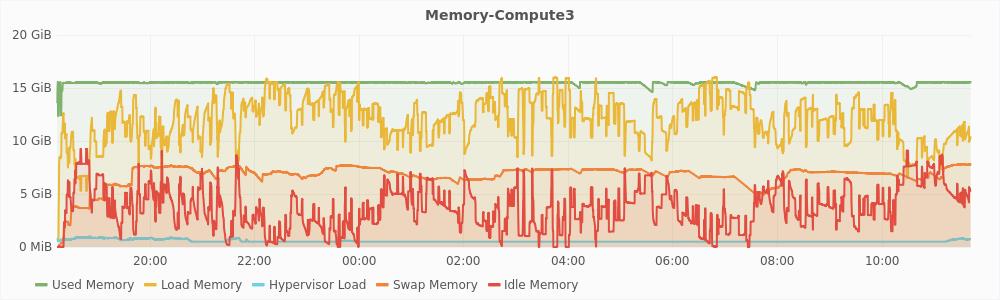
\includegraphics[width=\textwidth]{mem-compute3.png}
   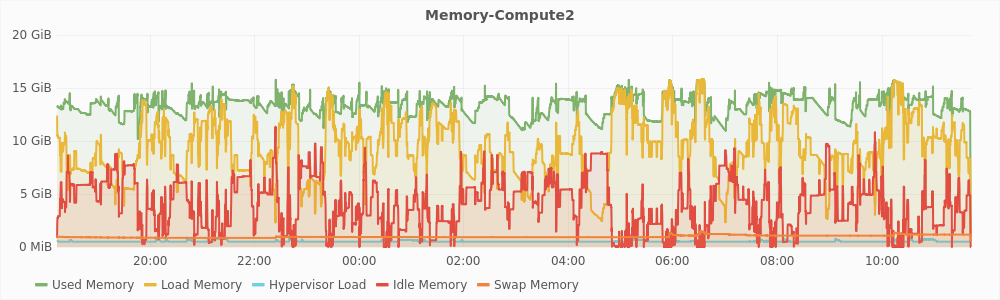
\includegraphics[width=\textwidth]{mem-compute2.png}
  \caption{Graphs showing different memory metrics of compute3 (autoballooning disabled) and compute 2 (autoballooning enabled). X-axis represents the time at which the value was recorded, Y-axis shows the value.}\label{fig:mem}
\end{sidewaysfigure}

Figure \ref{fig:cpu} shows the CPU usage of compute2 and compute3 plotted against time. In the graph, a few hours after starting the experiment, the CPU usage of compute3 is consistently low, while compute2 makes better use of the CPU. This is because of high levels of swap on compute 3. The mcf and usemem workloads spend more time in performing I/O and hence are not able to utilize the CPU efficiently.

\begin{sidewaysfigure}[!htbp]
  \centering
  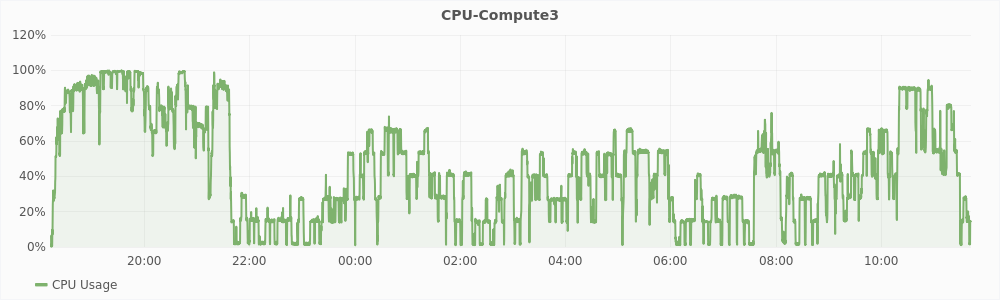
\includegraphics[width=\textwidth]{cpu-compute3.png}
  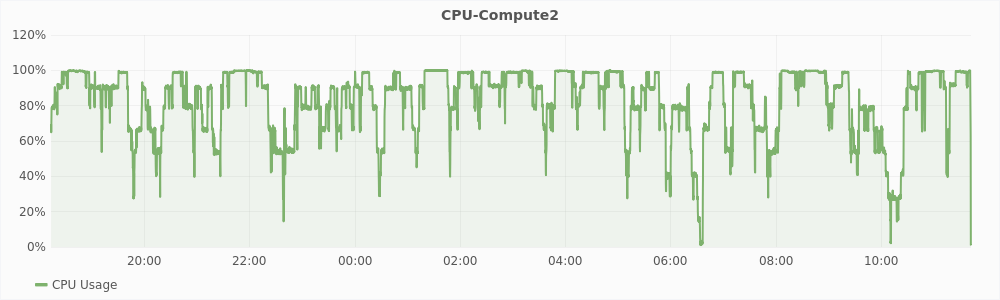
\includegraphics[width=\textwidth]{cpu-compute2.png}
  \caption{Graphs showing cpu usage of compute3 (autoballooning disabled) and compute2 (autoballooning enabled). X-axis represents the time at which the value was recorded, Y-axis shows the value.}\label{fig:cpu}
\end{sidewaysfigure}
Table \ref{tab:count} lists the number of time each workload ran on both the machines. Libquantum and mcf are CPU intensive. On compute2, CPU intensive workloads ran 303 times compared to 287 times on compute3 in the same time interval. Mcf and usemem are memory intensive. On compute2, memory intensive workloads ran 357 times compared to 289 times on compute 3 in the same time interval. It clearly shows that there was better utilization of the CPU and memory resources on compute2 resulting in a better overall throughput. 

\begin{table}[hbt]
\caption{Number of times each workload ran during the experiment}
\label{tab:count}
\begin{center}
\begin{tabularx}{0.91\textwidth}{XXX}
\hline\noalign{\smallskip}
Workload & Count-compute3 & Count-compute2\\
\noalign{\smallskip}
\hline
\noalign{\smallskip}
libquantum & 153 & 198\\

mcf & 134 & 105 \\

usemem & 155 & 252 \\
\hline
\end{tabularx}
\end{center}
\end{table}


\begin{sidewaysfigure}[!htbp]
  \centering
  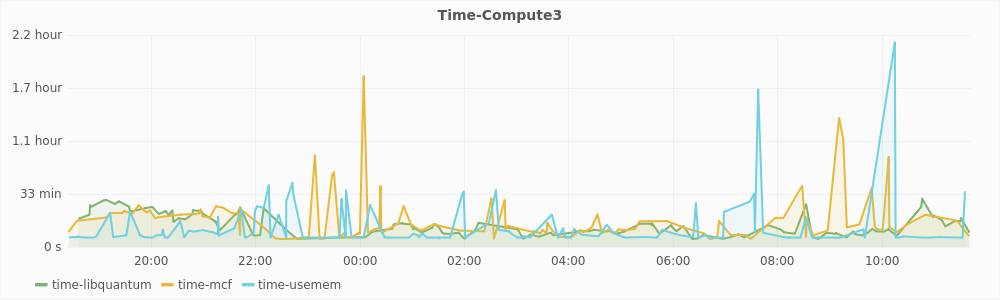
\includegraphics[width=\textwidth]{time-compute3.png}
  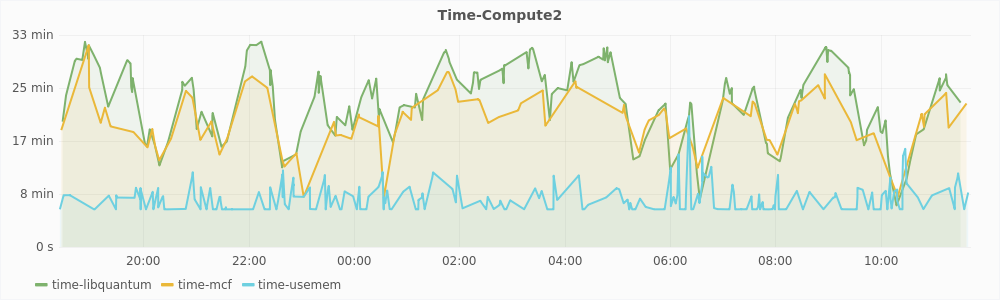
\includegraphics[width=\textwidth]{time-compute2.png}
  \caption{Graphs showing the time taken by different workloads on the two hosts. The values greater than two hours have been filtered out from the compute3 graph for the sake of visibility. X-axis represents the time at which the value was recorded, Y-axis shows the value.}\label{fig:time}
\end{sidewaysfigure}


\begin{table}[!htbp]
\caption{Mean time taken by each workload to run}
\label{tab:mean}
\begin{center}
\begin{tabularx}{0.91\textwidth}{XXX}
\hline\noalign{\smallskip}
Workload & Mean-compute3 & Mean-compute2\\
\noalign{\smallskip}
\hline
\noalign{\smallskip}
libquantum & 14.5 min & 23.7 min\\

mcf & 39.6 min & 20.3 min\\

usemem & 12.8 min & 7.9 min \\
\hline
\end{tabularx}
\end{center}
\end{table}

The graphs in Figure \ref{fig:time} show the time it took for the workloads to run plotted against the time at which the workload completed. In the graph for compute3, we can see that the time to complete the memory intensive workloads - mcf and usemem can grow to more than two hours while it always remains below 33 minutes on compute2. On top of this, some of the very large values have been filtered out from the graph of compute3. There were three such values for the mcf benchmark, which were greater than 9 hours. On the contrary, the libquantum workload performs better on compute3. This is because libquantum does not require much memory and the CPU on compute3 is relatively free because the other workloads do not utilize it well.
Table \ref{tab:mean} shows the mean time it took for the workloads to run. As expected, the libquantum performs better on compute3 while the other workloads perform better on compute2. But mean time is not a good metric to compare the effectiveness of autoballooning. Throughput is a better metric.

\subsection{Analyzing CPU Hotspot Detection}

\begin{sidewaysfigure}[!htbp]
  \centering
  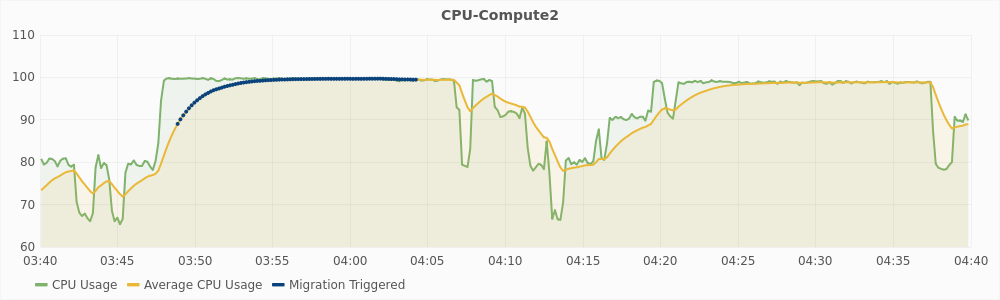
\includegraphics[width=\textwidth]{cpu-migration.png}
  \caption{CPU usage of compute2 during one hour of the experiment. Blue dots show the points at which migration was triggered. X-axis represents the time at which the value was recorded, Y-axis shows the value in \%}\label{fig:cpu-mig}
\end{sidewaysfigure}

The graph in Figure \ref{fig:cpu-mig} shows the CPU usage of compute2 for one hour during the experiment. The blue dots represent the instances at which migration was triggered. Migration was disabled for this experiment, so no machines was actually migrated out of this host. In the graph, the CPU usage is 100\% in two intervals. First interval is from around time 3:47 to 4:06 (interval1) and the second interval is from around 4:21 to 4:38 (interval2). However, migration is triggered only during interval1. This implies that there was a hotspot due to CPU utilization only during interval1 and not during interval2.

\begin{figure}[!htbp]
  \centering
  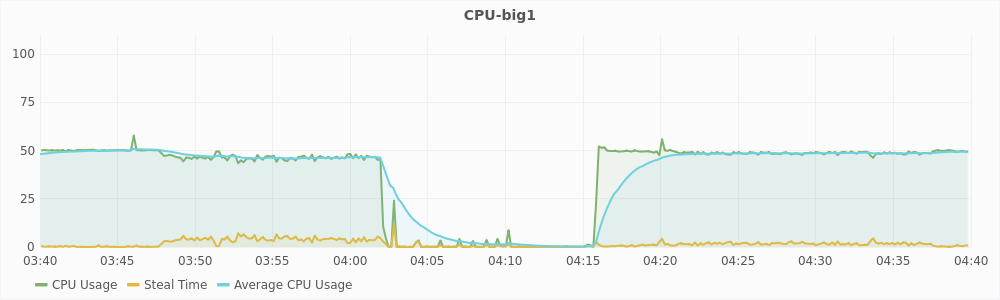
\includegraphics[width=\textwidth]{cpu-big1.png}
  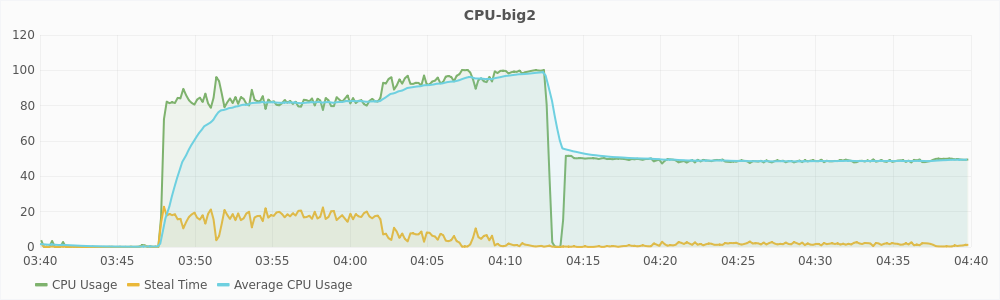
\includegraphics[width=\textwidth]{cpu-big2.png}
  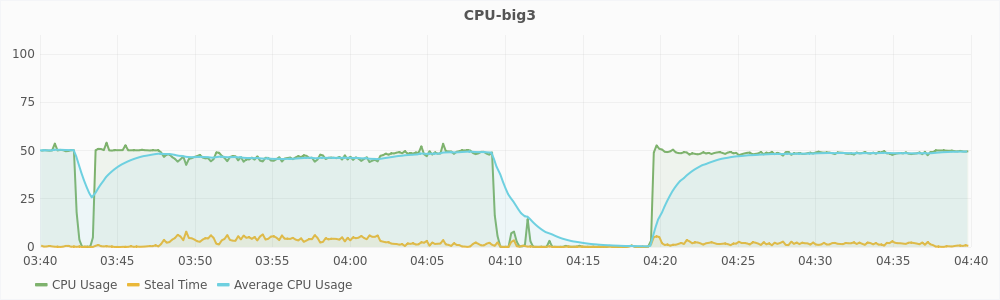
\includegraphics[width=\textwidth]{cpu-big3.png}
  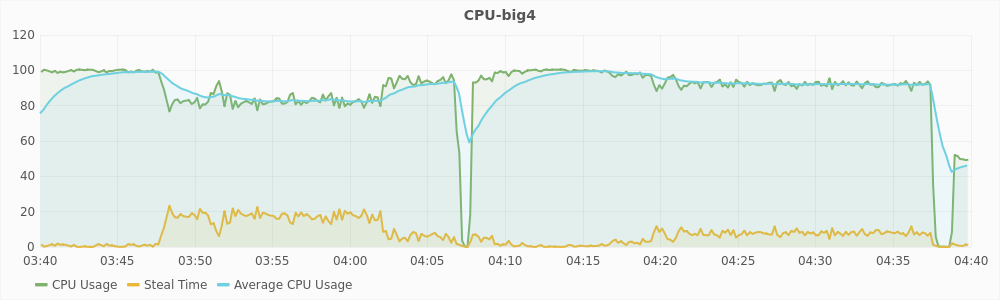
\includegraphics[width=\textwidth]{cpu-big4.png}
  \caption{CPU usage of all the large VMs on compute2 during 1 hour of the experiment. X-axis represents the time at which the value was recorded, Y-axis shows the value in \%}\label{fig:cpu-large}
\end{figure}

\begin{figure}[!htbp]
  \centering
  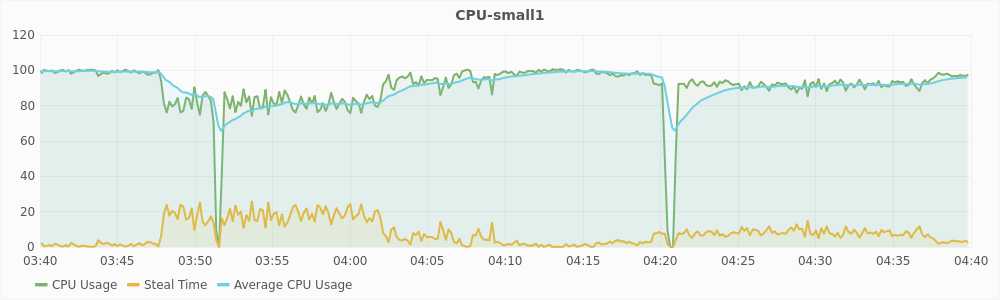
\includegraphics[width=\textwidth]{cpu-small1.png}
  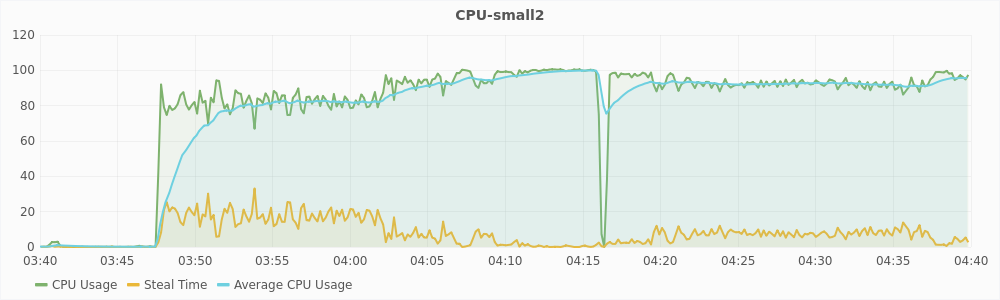
\includegraphics[width=\textwidth]{cpu-small2.png}
  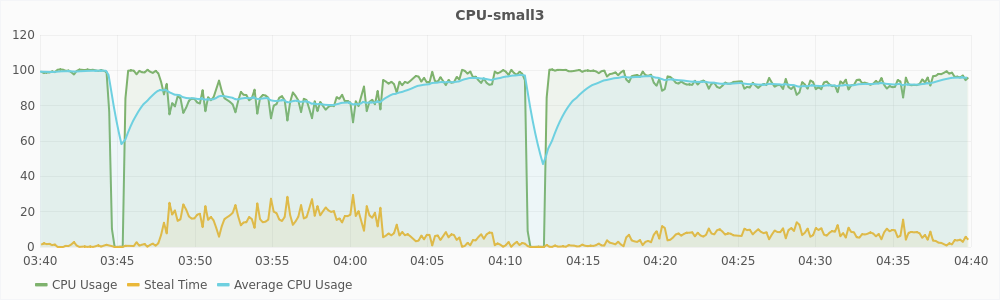
\includegraphics[width=\textwidth]{cpu-small3.png}
  \caption{CPU usage of all the small VMs on compute2 during 1 hour of the experiment. X-axis represents the time at which the value was recorded, Y-axis shows the value in \%}\label{fig:cpu-small}
\end{figure}

The graphs in Figure \ref{fig:cpu-large} and \ref{fig:cpu-small} show the CPU usage and steal time of individual virtual machines on compute2 during that one hour. For a large virtual machines, 100\% CPU usage implies that it is using two vCPUs completely and 50\% CPU usage implies that it is using only one of its two vCPUs. For a small virtual machines, 100\% CPU usage means that it is using its only vCPU completely. From the graphs, we can see that during interval1, large virtual machines are trying to use 6 vCPUs and the small virtual machines are trying to use 3 vCPUs, which is a total of 9 vCPUs. The host has only 8 physical CPUs and hence, it is overloaded. This also reflected in the steal time of the individual VMs which is higher than 10\% during interval1. During interval2, a total of 8 vCPUs are being used, which is equal to the number of the physical CPUs, and hence there is no overload. The steal time of the VMs are also low and migration is not triggered. These observations show that steal time is an appropriate metric for determining CPU hotspots.



\subsection{Analyzing the CUSUM algorithm}
Figure \ref{fig:etcd} shows a graph of one hour time duration of the experiment. The red dots in the graph mark the different points at which etcd was updated with the value of used memory for the host compute2. It is evident from the graph that the algorithm is successful in filtering sudden changes in the value of load memory and only updates etcd when the load profile has changed. In the one hour time duration, etcd was updated 13 times. Without the filtering algorithm, etcd would have been updated once in every 10 seconds i.e.\ 360 time in an hour, which is about 28 times more than the filtering algorithm. Overall during the 17 hour run of the experiment, etcd was updated just 266 times.
\begin{sidewaysfigure}[!htbp]
  \centering
  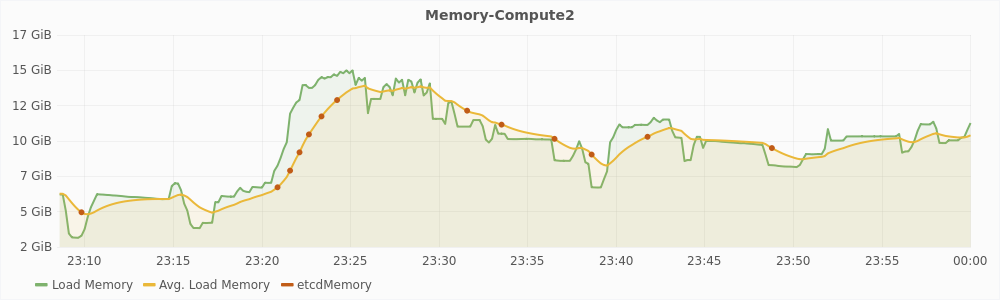
\includegraphics[width=\textwidth]{etcd-mem.png}
  \caption{Graphs showing the points at which etcd is updated. X-axis represents the time at which the value was recorded, Y-axis shows the value.}\label{fig:etcd}
\end{sidewaysfigure}

\subsection{Memory and CPU Footprint of DRS}
\begin{figure}[!htbp]
  \centering
  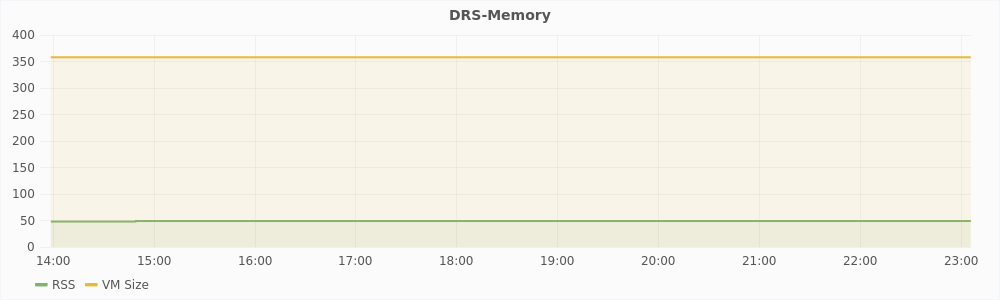
\includegraphics[width=\textwidth]{mem-self.png}
  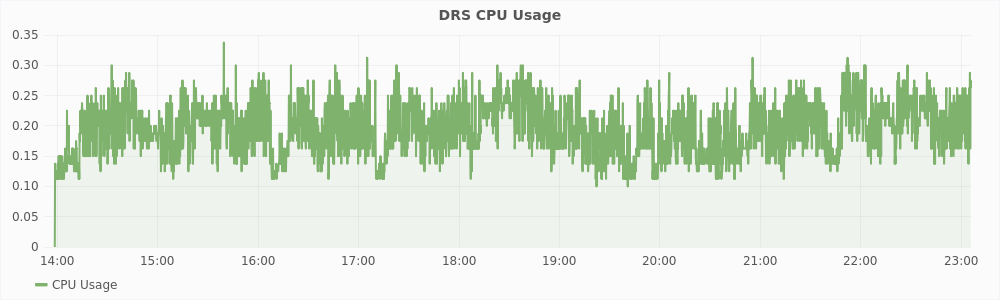
\includegraphics[width=\textwidth]{cpu-self.png}
  \caption{Graphs showing the CPU and memory used by the DRS. The memory usage is shown in MBs abd CPU usage in \%}\label{fig:self}
\end{figure}

Graphs in Figure \ref{fig:self} show the resource usage statistics of the DRS algorithm. As we can see, the CPU usage is always less then 0.35\% which is almost negligible. The memory used by the DRS algorithm is 50MB with the entire virtual memory size of the software being just 350MB.

\section*{Summary}
In this chapter, we described our experimental setup and compared the resource utilization without autoballooning with the case when autoballooning was enabled. We looked at the effectiveness of steal time in identifying CPU hotspots. We also saw the performance of the CUSUM algorithm which is used to filter sudden changes in the resource usage from affecting decision making of the DRS algorithm. We also looked at the resources consumed by our implementation of the DRS algorithm.
